\documentclass[english,floatsintext,man]{apa6}

\usepackage{amssymb,amsmath}
\usepackage{ifxetex,ifluatex}
\usepackage{fixltx2e} % provides \textsubscript
\ifnum 0\ifxetex 1\fi\ifluatex 1\fi=0 % if pdftex
  \usepackage[T1]{fontenc}
  \usepackage[utf8]{inputenc}
\else % if luatex or xelatex
  \ifxetex
    \usepackage{mathspec}
    \usepackage{xltxtra,xunicode}
  \else
    \usepackage{fontspec}
  \fi
  \defaultfontfeatures{Mapping=tex-text,Scale=MatchLowercase}
  \newcommand{\euro}{€}
\fi
% use upquote if available, for straight quotes in verbatim environments
\IfFileExists{upquote.sty}{\usepackage{upquote}}{}
% use microtype if available
\IfFileExists{microtype.sty}{\usepackage{microtype}}{}

% Table formatting
\usepackage{longtable, booktabs}
\usepackage{lscape}
% \usepackage[counterclockwise]{rotating}   % Landscape page setup for large tables
\usepackage{multirow}		% Table styling
\usepackage{tabularx}		% Control Column width
\usepackage[flushleft]{threeparttable}	% Allows for three part tables with a specified notes section
\usepackage{threeparttablex}            % Lets threeparttable work with longtable

% Create new environments so endfloat can handle them
% \newenvironment{ltable}
%   {\begin{landscape}\begin{center}\begin{threeparttable}}
%   {\end{threeparttable}\end{center}\end{landscape}}

\newenvironment{lltable}
  {\begin{landscape}\begin{center}\begin{ThreePartTable}}
  {\end{ThreePartTable}\end{center}\end{landscape}}




% The following enables adjusting longtable caption width to table width
% Solution found at http://golatex.de/longtable-mit-caption-so-breit-wie-die-tabelle-t15767.html
\makeatletter
\newcommand\LastLTentrywidth{1em}
\newlength\longtablewidth
\setlength{\longtablewidth}{1in}
\newcommand\getlongtablewidth{%
 \begingroup
  \ifcsname LT@\roman{LT@tables}\endcsname
  \global\longtablewidth=0pt
  \renewcommand\LT@entry[2]{\global\advance\longtablewidth by ##2\relax\gdef\LastLTentrywidth{##2}}%
  \@nameuse{LT@\roman{LT@tables}}%
  \fi
\endgroup}


  \usepackage{graphicx}
  \makeatletter
  \def\maxwidth{\ifdim\Gin@nat@width>\linewidth\linewidth\else\Gin@nat@width\fi}
  \def\maxheight{\ifdim\Gin@nat@height>\textheight\textheight\else\Gin@nat@height\fi}
  \makeatother
  % Scale images if necessary, so that they will not overflow the page
  % margins by default, and it is still possible to overwrite the defaults
  % using explicit options in \includegraphics[width, height, ...]{}
  \setkeys{Gin}{width=\maxwidth,height=\maxheight,keepaspectratio}
\ifxetex
  \usepackage[setpagesize=false, % page size defined by xetex
              unicode=false, % unicode breaks when used with xetex
              xetex]{hyperref}
\else
  \usepackage[unicode=true]{hyperref}
\fi
\hypersetup{breaklinks=true,
            pdfauthor={},
            pdftitle={Who are you trying to impress? When does showing skin increase attractiveness in social media.},
            colorlinks=true,
            citecolor=blue,
            urlcolor=blue,
            linkcolor=black,
            pdfborder={0 0 0}}
\urlstyle{same}  % don't use monospace font for urls

\setlength{\parindent}{0pt}
%\setlength{\parskip}{0pt plus 0pt minus 0pt}

\setlength{\emergencystretch}{3em}  % prevent overfull lines

\ifxetex
  \usepackage{polyglossia}
  \setmainlanguage{}
\else
  \usepackage[english]{babel}
\fi

% Manuscript styling
\captionsetup{font=singlespacing,justification=justified}
\usepackage{csquotes}
\usepackage{upgreek}

 % Line numbering
  \usepackage{lineno}
  \linenumbers


\usepackage{tikz} % Variable definition to generate author note

% fix for \tightlist problem in pandoc 1.14
\providecommand{\tightlist}{%
  \setlength{\itemsep}{0pt}\setlength{\parskip}{0pt}}

% Essential manuscript parts
  \title{Who are you trying to impress? When does showing skin increase
attractiveness in social media.}

  \shorttitle{facebook}


  \author{Nathaniel Phillips\textsuperscript{1}~\& Joerg Rieskamp\textsuperscript{1}}

  \def\affdep{{"", ""}}%
  \def\affcity{{"", ""}}%

  \affiliation{
    \vspace{0.5cm}
          \textsuperscript{1} University of Basel  }

 % If no author_note is defined give only author information if available
      \newcounter{author}
                              \authornote{
          Correspondence concerning this article should be addressed to Nathaniel Phillips
          , Missionsstrasse 62A 4053 Basel Switzerland .
           E-mail: \href{mailto:nathaniel.phillips@unibas.ch}{\nolinkurl{nathaniel.phillips@unibas.ch}} 
          }
                                  
  \note{The first author is at the Economic Psychology department at the
University of Basel.}

  \abstract{Does the presence of skin help or hurt dateability ratings in social
media profiles? To answer this question, we had 1,000 participants
access how dateable people were based on their Facebook profiles. We
found strong evidence for an interaction between sex and skin. When men
did not wear shirts, their dateability scored decreased. For women, the
effect was reversed.}
  \keywords{apa, R, markdown \\

    \indent Word count: X
  }





\usepackage{amsthm}
\newtheorem{theorem}{Theorem}
\newtheorem{lemma}{Lemma}
\theoremstyle{definition}
\newtheorem{definition}{Definition}
\newtheorem{corollary}{Corollary}
\newtheorem{proposition}{Proposition}
\theoremstyle{definition}
\newtheorem{example}{Example}
\theoremstyle{remark}
\newtheorem*{remark}{Remark}
\begin{document}

\maketitle

\setcounter{secnumdepth}{0}



Nudity has long been studied in the psychological literature (Alexander
\& Judd, 1986; LaTour, 1990), usually in the context of advertising.
Social media sites such as Facebook are ways for people to express and
advertise themselves to their peers. People's behavior on Facebook has
been measured with respect to personality types. For example, Ross et
al. (2009) found that personality factors were not very influential on
Facebook use.

Similar to social media sites such as Facebook, online dating has become
a popular medium for people to connect. For example Ellison, Heino, and
Gibbs (2006) studied how people present themselves in online dating
profiles.

However, no researchers have studied the connection between nudity and
social media. The purpose of this study is to determine to what extent
nudity affects perceptions of dateability in social media. In the study,
we asked single participants to view Facebook profiles of people that
were either wearing a shirt or not in their profile picture. They then
rated how dateable each person was.

\section{Method}\label{method}

\subsection{Participants}\label{participants}

1000 participants were recruited from the University of Basel to
participate in the study in exchange for 5 Swiss Francs. The mean age
was 22 and there were 479 females.

\subsection{Materials}\label{materials}

Each profile was displayed as a static screenshot. The primary measure
was a dateability score on a scale from 0 to 100.

\subsection{Procedure}\label{procedure}

Participants viewed a static profile for 60 seconds. When the profile
disappeared, participants gave their ratings.

\section{Results}\label{results}

A histogram of dateability scores is presented in Figure 1. The mean
dateability score was 54.

\begin{figure}[htbp]
\centering
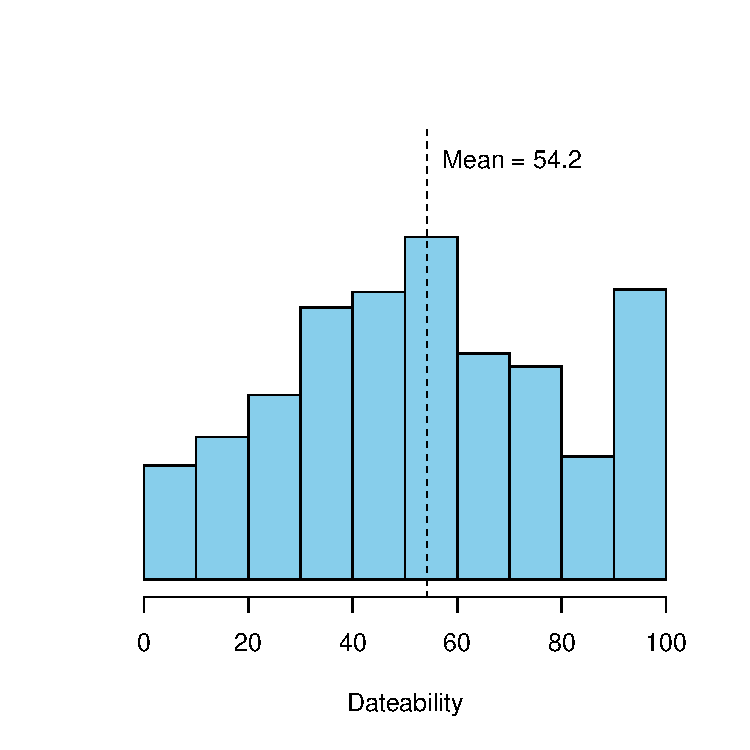
\includegraphics{02-papaja-example-article-nathaniel-phillips_files/figure-latex/unnamed-chunk-3-1.pdf}
\caption{\label{fig:unnamed-chunk-3}Distribution of dateability scores}
\end{figure}

Next we looked to see if there was a relationship between whether a
person wore a shirt in their prifle photo or not on their dateability
scores. A pirateplot showing distributions of scores split by sex and
whether people wore a shirt or not is presented in Figure 2:

\begin{figure}[htbp]
\centering
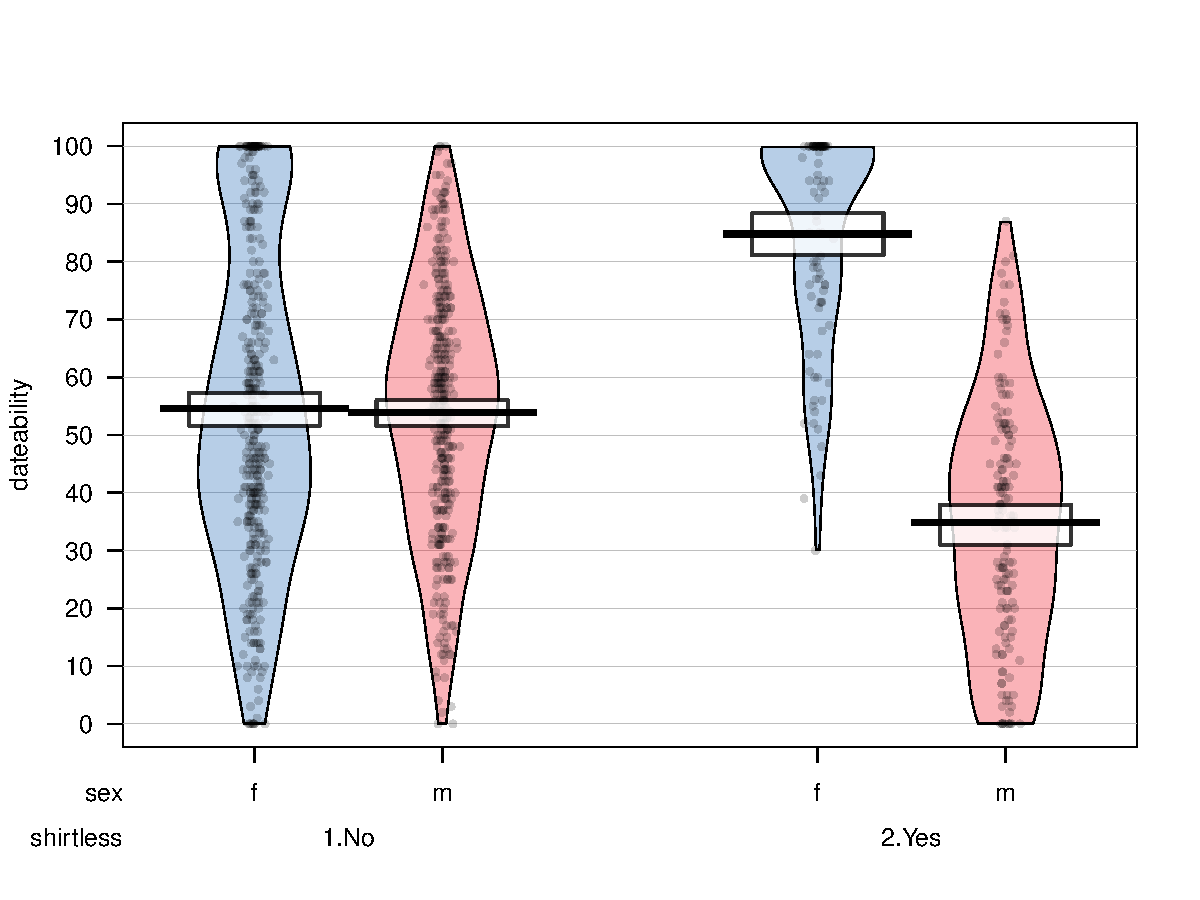
\includegraphics{02-papaja-example-article-nathaniel-phillips_files/figure-latex/unnamed-chunk-4-1.pdf}
\caption{\label{fig:unnamed-chunk-4}Distribution of dateability scores by
sex and shirt. The data clearly show that not wearing a shirt increases
scores for women, but decreases scores for men.}
\end{figure}

Descriptively, the data show a clear interaction between sex and shirt
wearing. To test this interaction, we conducted an ANOVA. The ANOVA
showed a significant interaction between sex and shirt wearing on scores
(see Table 1).

\begin{table}[tbp]
\begin{center}
\begin{threeparttable}
\caption{\label{tab:unnamed-chunk-5}ANOVA on dateability ratings}
\begin{tabular}{lllllll}
\toprule
Effect & \multicolumn{1}{c}{$F$} & \multicolumn{1}{c}{$\mathit{df}_1$} & \multicolumn{1}{c}{$\mathit{df}_2$} & \multicolumn{1}{c}{$\mathrm{MSE}$} & \multicolumn{1}{c}{$p$} & \multicolumn{1}{c}{$\eta^2_G$}\\
\midrule
Sex & 62.69 & 1 & 996 & 582.46 & < .001 & .059\\
Shirtless & 0.42 & 1 & 996 & 582.46 & .515 & .000\\
Sex $\times$ Shirtless & 183.79 & 1 & 996 & 582.46 & < .001 & .156\\
\bottomrule
\end{tabular}
\end{threeparttable}
\end{center}
\end{table}

The relationship between age and dateability is shown in Figure 2. A
correlation test showed that the relationship was non-significant
(t(998) = 1.5 p = 0.13)

\begin{figure}[htbp]
\centering
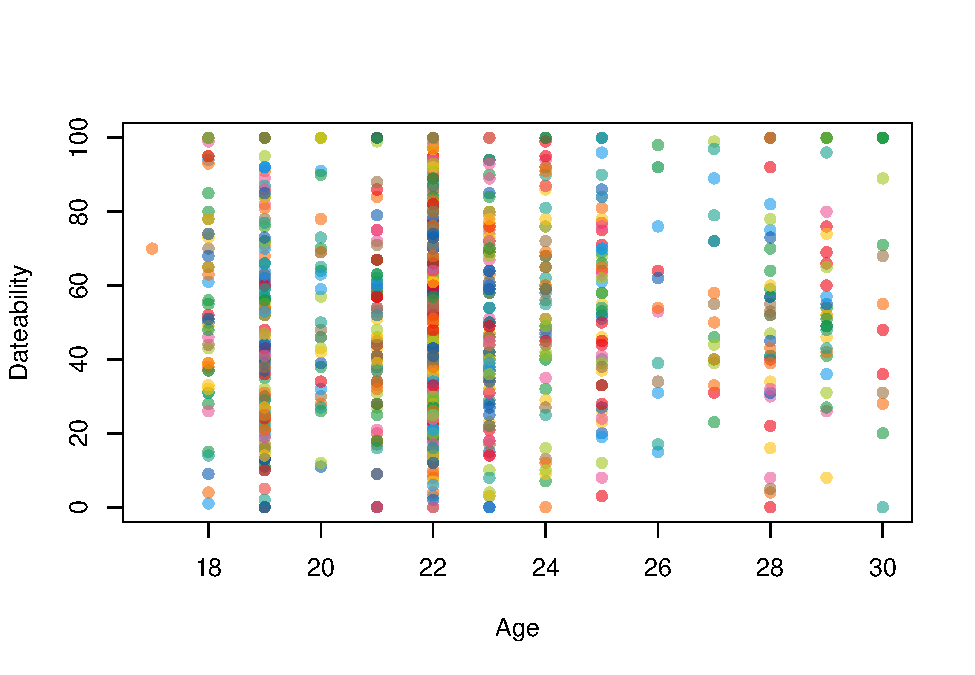
\includegraphics{02-papaja-example-article-nathaniel-phillips_files/figure-latex/unnamed-chunk-7-1.pdf}
\caption{\label{fig:unnamed-chunk-7}Relationship between age and
dateability. The relationship was not significant.}
\end{figure}

\section{Discussion}\label{discussion}

This fake study showed an interesting interaction between nudity and sex
on attraction in social media profiles. More (real) research is needed.

\section{References}\label{references}

\setlength{\parindent}{-0.5in} \setlength{\leftskip}{0.5in}
\setlength{\parskip}{8pt}

\hypertarget{refs}{}
\hypertarget{ref-alexander1986differences}{}
Alexander, M. W., \& Judd, B. B. (1986). Differences in attitudes toward
nudity in advertising. \emph{Psychology: A Journal of Human Behavior}.

\hypertarget{ref-ellison2006managing}{}
Ellison, N., Heino, R., \& Gibbs, J. (2006). Managing impressions
online: Self-presentation processes in the online dating environment.
\emph{Journal of Computer-Mediated Communication}, \emph{11}(2),
415--441.

\hypertarget{ref-latour1990female}{}
LaTour, M. S. (1990). Female nudity in print advertising: An analysis of
gender differences in arousal and ad response. \emph{Psychology \&
Marketing}, \emph{7}(1), 65--81.

\hypertarget{ref-ross2009personality}{}
Ross, C., Orr, E. S., Sisic, M., Arseneault, J. M., Simmering, M. G., \&
Orr, R. R. (2009). Personality and motivations associated with facebook
use. \emph{Computers in Human Behavior}, \emph{25}(2), 578--586.






\end{document}
